% Made up for the tikra benchmark.
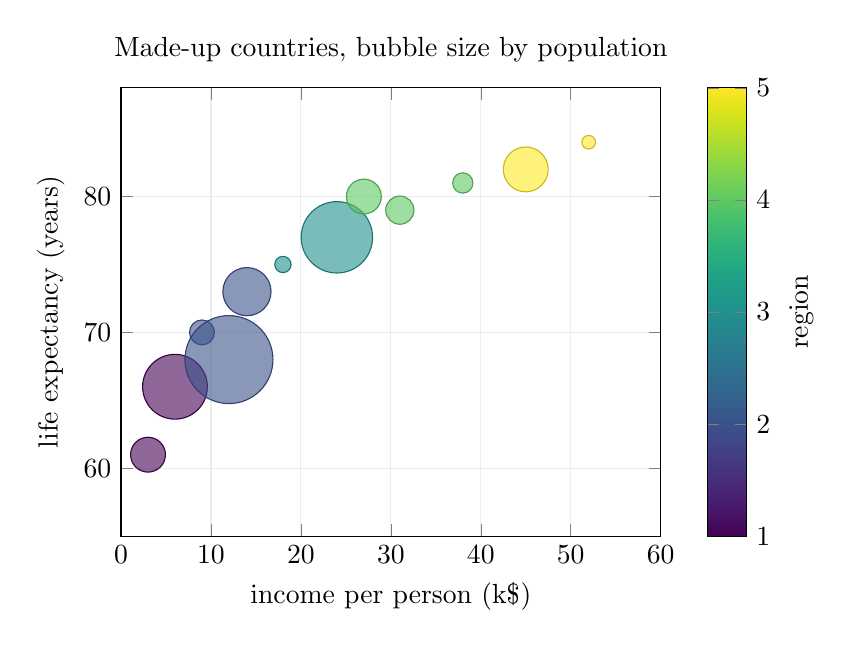
\begin{tikzpicture}
\begin{axis}[xlabel={income per person (k\$)}, ylabel={life expectancy (years)},
    title={Made-up countries, bubble size by population}, xmin=0, xmax=60, ymin=55, ymax=88,
    grid=major, grid style={gray!15}, colormap/viridis, colorbar, colorbar style={ylabel=region}]
  \addplot[scatter, only marks, scatter src=explicit, mark=*,
      visualization depends on={\thisrow{pop} \as \pop},
      scatter/@pre marker code/.append style={/tikz/mark size={1.5pt+0.12pt*\pop}},
      mark options={fill opacity=0.6, draw=black!60}]
    table[x=inc, y=life, meta=reg] {
      inc life pop reg
      3   61   40  1
      6   66   85  1
      9   70   25  2
      14  73   60  2
      18  75   12  3
      24  77   95  3
      31  79   30  4
      38  81   18  4
      45  82   55  5
      52  84   8   5
      12  68   120 2
      27  80   40  4
    };
\end{axis}
\end{tikzpicture}
